\documentclass{article}
\usepackage{amsmath,amsfonts,amssymb,amsthm, mathrsfs, mathtools, tikz, float}
\usepackage{listings}
\usepackage{xcolor} % Required for custom colors
\usepackage{amsmath}
\usepackage{pgfplots}

\pgfplotsset{compat=1.17}

% Define custom colors
\definecolor{codegreen}{rgb}{0,0.6,0}
\definecolor{codegray}{rgb}{0.5,0.5,0.5}
\definecolor{codepurple}{rgb}{0.58,0,0.82}
\definecolor{backcolour}{rgb}{0.95,0.95,0.92}

% Setup the style for code listings
\lstdefinestyle{mystyle}{
    backgroundcolor=\color{backcolour},   
    commentstyle=\color{codegreen},
    keywordstyle=\color{magenta},
    numberstyle=\tiny\color{codegray},
    stringstyle=\color{codepurple},
    basicstyle=\ttfamily\footnotesize,
    breakatwhitespace=false,         
    breaklines=true,                 
    captionpos=b,                    
    keepspaces=true,                 
    numbers=left,                    
    numbersep=5pt,                  
    showspaces=false,                
    showstringspaces=false,
    showtabs=false,                  
    tabsize=2
}

\lstset{style=mystyle}
\usetikzlibrary{graphs,calc} % LATEX and plain TEX
\title{Algorithmics: Project}
\author{Martin Stuwe, 676421}

\begin{document}
\maketitle

\section{Introduction}
The Nordic Film Days is an annual event that attracts movie enthusiasts from around the world. To make the most of this festival, we faced a challenging problem: how to create a schedule that allows us to watch as many different films as possible, optimize our viewing experience by selecting high-rated films, and minimize travel time between venues. In this report, we present our approach and implementation of this scheduling problem.
\section{Problem Description}
The Nordic Film Days involve simultaneous screenings of various films at different venues. Our goal is to create a schedule that adheres to the following criteria:
\begin{enumerate}
\item Maximize the number of different films watched (no duplicates).
\item Optimize the overall film rating based on IMDb rankings.
\item Minimize travel time between venues, considering delays caused by location changes and a one-minute grace period for joining screenings.
\end{enumerate}
We are provided with data on films, including their title, weekday, start time, duration, location, and rating. Additionally, we have information about travel times between venues, as shown in Table 1.


\section{Methodology}
To solve this scheduling problem, we implemented a Python program using the PuLP package. The key steps in our methodology include:
\begin{enumerate}
\item Data preprocessing: Reading film data from CSV files and organizing it into appropriate data structures.
\item Linear programming formulation: Defining decision variables, the objective function, and constraints to maximize film ratings while avoiding overlaps and considering travel times.
\item Solving the linear program: Using PuLP to find the optimal film schedule that satisfies all constraints.
\end{enumerate}

We maximize the summation over all showings multiplied by their respective rating.
Subject to the contraints, that each movie can only be watched once and that overlapping movies cannot be watched.
Our preprocessing steps in our python script determine with the help of a mapping of cinema tuples for the distances, which movies overlap to formulate the respective constraints.
The integer program for one of the small datasets is:

\begin{align*}
    &\text{MAXIMIZE }
        5.9 \cdot \text{Showing}_0 + 5.9 \cdot \text{Showing}_1 + 5.8 \cdot \text{Showing}_{10} +\\
        &3.8 \cdot \text{Showing}_{11} + 5.9 \cdot \text{Showing}_{12} + \\
        & 5.7 \cdot \text{Showing}_{13} + 5.9 \cdot \text{Showing}_{14} + \\
        &5.9 \cdot \text{Showing}_2 + 5.8 \cdot \text{Showing}_3 + 5.9 \cdot \text{Showing}_4 + \\
        & 5.8 \cdot \text{Showing}_5 + 5.9 \cdot \text{Showing}_6 + 5.9 \cdot \text{Showing}_7 + 4.3 \cdot \text{Showing}_8 + 5.9 \cdot \text{Showing}_9 + 0.0\\
    \text{SUBJECT TO} & \\
    & \text{Showing}_7 + \text{Showing}_8 \leq 1 \\
    & \text{Showing}_3 + \text{Showing}_5 \leq 1 \\
    & \text{Showing}_6 \leq 1 \\
    & \text{Showing}_8 \leq 1 \\
    & \text{Showing}_2 + \text{Showing}_7 \leq 1 \\
    & \text{Showing}_0 + \text{Showing}_{14} + \text{Showing}_4 + \text{Showing}_9 \leq 1 \\
    &  \text{Showing}_1 + \text{Showing}_{12} \leq 1 \\
    & \text{Showing}_{13} \leq 1 \\
    &  \text{Showing}_{11} \leq 1 \\
    &  \text{Showing}_{10} \leq 1 \\
    & \text{Showing}_i \in \{0,1\} \quad \forall i \in \{0,1,2,3,4,5,6,7,8,9,10,11,12,13,14\}
\end{align*}


We use binary variables to decide whether we watch a movie or not. To avoid watching the same movie, we sum the respective variables for the same films at different locations/times and require that the sum be less than or equal to 1. The same logic applies to overlapping movies.

\section{Implementation}
Our Python implementation effectively handles the scheduling problem for multiple datasets. We create LP variables, define the objective function to maximize the overall rating, and set up constraints to ensure no overlaps and no duplicates. We also consider travel times and delays when constructing the schedule. Our implementation generates output files containing the results for each dataset.
The implementation can be found in main.py.

\section{Results}
We successfully solved the scheduling problem for various datasets, providing optimal movie schedules that maximize IMDb ratings. We recorded the objective values and runtime for each dataset. The results are stored in output files for further analysis.



\begin{figure}
    \centering
    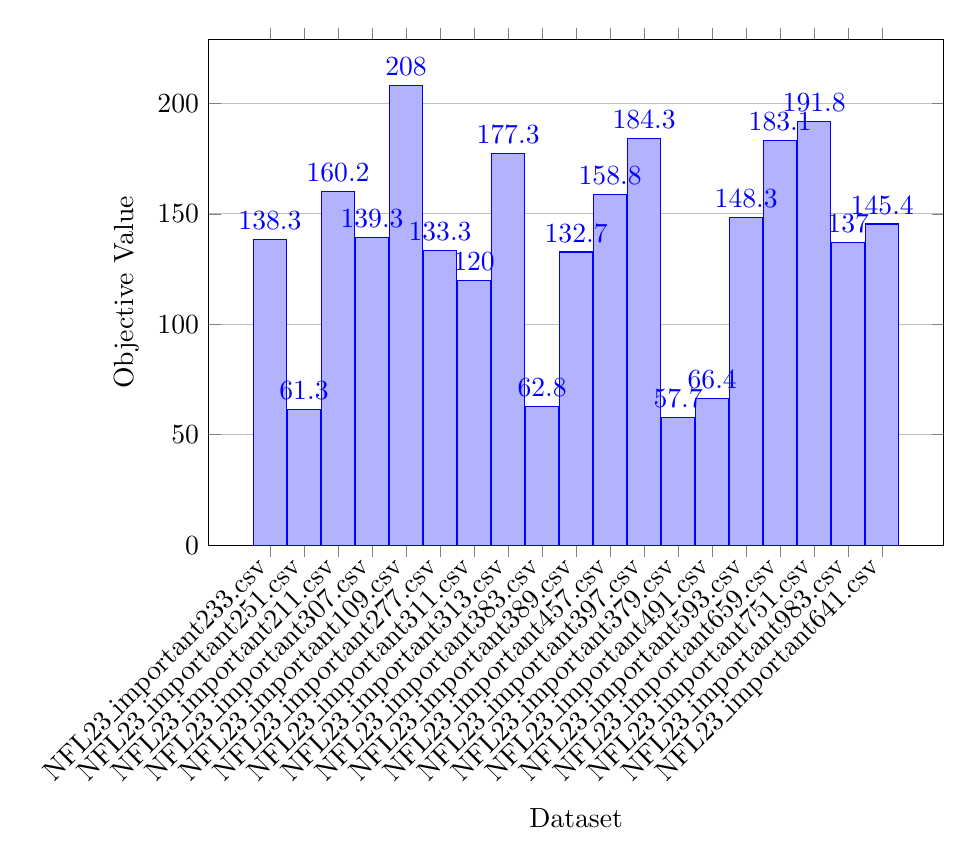
\begin{tikzpicture}
    \begin{axis}[
        ybar,
        xlabel={Dataset},
        ylabel={Objective Value},
        symbolic x coords={
            NFL23\_important233.csv,
            NFL23\_important251.csv,
            NFL23\_important211.csv,
            NFL23\_important307.csv,
            NFL23\_important109.csv,
            NFL23\_important277.csv,
            NFL23\_important311.csv,
            NFL23\_important313.csv,
            NFL23\_important383.csv,
            NFL23\_important389.csv,
            NFL23\_important457.csv,
            NFL23\_important397.csv,
            NFL23\_important379.csv,
            NFL23\_important491.csv,
            NFL23\_important593.csv,
            NFL23\_important659.csv,
            NFL23\_important751.csv,
            NFL23\_important983.csv,
            NFL23\_important641.csv
        },
        xtick=data,
        x tick label style={rotate=45,anchor=east},
        nodes near coords,
        nodes near coords align={vertical},
        bar width=12pt,
        enlarge x limits=0.1,
        ymin=0,
        ymajorgrids=true,
        width=0.9\textwidth,
        height=8cm
    ]
    \addplot coordinates {
        (NFL23\_important233.csv, 138.3)
        (NFL23\_important251.csv, 61.3)
        (NFL23\_important211.csv, 160.2)
        (NFL23\_important307.csv, 139.3)
        (NFL23\_important109.csv, 208.0)
        (NFL23\_important277.csv, 133.3)
        (NFL23\_important311.csv, 120.0)
        (NFL23\_important313.csv, 177.3)
        (NFL23\_important383.csv, 62.8)
        (NFL23\_important389.csv, 132.7)
        (NFL23\_important457.csv, 158.8)
        (NFL23\_important397.csv, 184.3)
        (NFL23\_important379.csv, 57.7)
        (NFL23\_important491.csv, 66.4)
        (NFL23\_important593.csv, 148.3)
        (NFL23\_important659.csv, 183.1)
        (NFL23\_important751.csv, 191.8)
        (NFL23\_important983.csv, 137.0)
        (NFL23\_important641.csv, 145.4)
    };
    \end{axis}
    \end{tikzpicture}
    \caption{Objective Values for Different Datasets}
\end{figure}

The respective runtimes are:

Dataset, Objective Value, Runtime (seconds)\\
NFL23\_important233.csv, 138.29999999999998, 0.16588878631591797\\
NFL23\_important251.csv, 61.3, 0.9919431209564209\\
NFL23\_important211.csv, 160.20000000000005, 0.2692911624908447\\
NFL23\_important307.csv, 139.29999999999998, 0.16666126251220703\\
NFL23\_important109.csv, 208.00000000000003, 0.4543285369873047\\
NFL23\_important277.csv, 133.29999999999998, 0.15290594100952148\\
NFL23\_important311.csv, 120.0, 0.12831354141235352\\
NFL23\_important313.csv, 177.30000000000004, 0.3689141273498535\\
NFL23\_important383.csv, 62.8, 0.9265275001525879\\
NFL23\_important389.csv, 132.7, 0.09563016891479492\\
NFL23\_important457.csv, 158.8, 0.19332408905029297\\
NFL23\_important397.csv, 184.29999999999995, 0.39622068405151367\\
NFL23\_important379.csv, 57.699999999999996, 0.239091157913208\\
NFL23\_important491.csv, 66.39999999999999, 1.3689641952514648\\
NFL23\_important593.csv, 148.3, 0.38736581802368164\\
NFL23\_important659.csv, 183.10000000000002, 0.2737290859222412\\
NFL23\_important751.csv, 191.80000000000004, 0.31435537338256836\\
NFL23\_important983.csv, 137.0, 0.17076683044433594\\
NFL23\_important641.csv, 145.4, 0.21124863624572754

\section{Conclusion}
In conclusion, our project for which we spend 10 hours tackles the scheduling problem for optimizing film festival attendance. We have implemented an efficient solution using linear programming techniques, Python, and the PuLP package. Our approach successfully meets the criteria of maximizing diverse film selection and optimizing overall rating while considering travel times. The results obtained demonstrate the effectiveness of our solution in creating optimal film schedules for the Nordic Film Days.


\end{document}

